\documentclass[a4paper,11pt]{article}
\usepackage[T1]{fontenc}
\usepackage[utf8]{inputenc}
\usepackage{lmodern}
\usepackage[italian]{babel}
\usepackage{graphicx}

\title{Relazione di Fisica Computazionale \\ 
    \textsc{Soluzione dell'equazione di Schroedinger con tecniche di diagonalizzazione numerica}
    }

\author{Rebecca Ghidoni \\ Alessandro Piras}

\begin{document}

\maketitle
% \tableofcontents

\begin{abstract}
Il progetto è volto a determinare gli autostati e le energie di un oscillatore armonico unidimensionale, a partire dall'equazione di Schroedinger del sistema. \\
Il problema sarà risolto con due diverse modalita, lavorando rispettivamente in spazio reale e in spazio reciproco. Entrambi i procedimenti puntano alla costruzione di una matrice i cui autovalori e autovettori siano facilmente ricavabili con metodi di diagonalizzazione.

\end{abstract}

\section*{Introduzione}
L'equazione di Schroedinger per una singola particella in un potenziale $V(x)$, unidimensionale e indipendente dal tempo, si può scrivere come 

\begin{equation}
\left[- \frac{\hbar^2}{2m}\frac{\partial^2}{\partial x^2} + V(x) \right] \Psi(x) = E\Psi(x)
\end{equation}

Nel caso preso in esame il potenziale sarà di tipo armonico, pertanto nell'equazione varrà $V(x) = \frac{m \omega^2}{2}x^2$. \\

La soluzione analitica di questo problema è nota, pertanto sarà facile confrontare le energie risultanti dal processo di diagonalizzazione con quelle calcolate, esprimibili come

\begin{equation}
E_n = (\frac{1}{2} + n) \hbar \omega, \quad n = 0, 1, 2, ...
\end{equation}

Per facilitare la lettura dei risultati è possibile scalare posizioni ed energie sulla base delle grandezze costanti presenti nell'equazione, così da ottenere valori nell'ordine dell'unità:

\begin{equation}
x \rightarrow \left( \frac{\hbar}{m\omega} \right)^\frac{1}{2} x
\end{equation}
\begin{equation} 
E \rightarrow \frac{E}{\hbar \omega}
\end{equation}

Tramite questa trasformazione si ottiene un'equazione di Schroedinger semplificata e quindi di più facile trattazione:

\begin{equation}
\left[ - \frac{\partial^2}{\partial x^2} + x^2 \right] \Psi(x) = 2E \Psi(x)
\end{equation}

dove ci si aspetta che le energie $E_n$ assumino valori interi o semi-interi e le funzioni d'onda si annullaino a poche unità di distanza dall'origine.

\section*{Task A}

Nel primo task lavoreremo in spazio reale, considerando un intervallo spaziale di ampliezza $L$, centrato nell'origine e suddiviso da una griglia di $N$ punti $x_k$. \\
Utilizziamo l'espressione alle differenze finite 
\begin{equation}
f'' = \frac{f(x-h) - 2f(x) + f(x + h)}{h^2}
\end{equation}
per riscrivere la derivata seconda della funzione d'onda. Inserendola nell'equazione si ottiene

\begin{equation}
- \frac{\psi_{k-1} - 2\psi_k + \psi_{k+1}}{h^2} + x^2_k \psi_k = 2E\psi_k
\end{equation}

dove $\psi_k = \psi(x_k)$ e $h$ è l'intervallo spaziale che separa due punti della griglia. \\
È stato possibile quindi ricavare un sistema di equazioni lineari in $N$ incognite, sinteticamente rappresentabili nella forma
\begin{equation}
H\psi = 2E\psi
\end{equation}

dove $\psi$ è il vettore colonna $(\psi_1, \psi_2, ..., \psi_N)^T$ e $H$ è una matrice tridiagonale, i cui elementi sono definiti da
\begin{equation}
H_{ij} = \left\{
\begin{array}{lr} 
-1/h^2,  & j = i - 1 \\
2/h^2 + x_i^2, & j = 1 \\
-1/h^2, & j = i + 1
\end{array}
\right.
\end{equation}

Diagonalizzando $H$ si possono così ottenere gli autovalori $E_n$ e le autofunzioni $\psi_n(x_k)$.

\newpage

\section*{Task B}

Un secondo metodo per risolvere l'equazione di Schrodinger consiste nello sviluppare le autofunzioni su di una base ortonormale $u_k(x)$, dove $k$ è un set di numeri quantici. \\
Una generica soluzione è pertanto scrivibile come combinazione lineari dei vettori della base:

\begin{equation}
\psi(x)= \sum_k  c_k u_k(x)
\end{equation}


La soluzione espressa in tale forma è sostituibile nell'equazione differenziale; moltiplicando scalarmente a sinistra per un generico vettore $u^*_{k'}(x)$ della base si ottiene un sistema di equazioni, la  cui $k'$-esima è scrivibile come
\begin{equation}
\sum_k c_k \left[ K_{k,k'} + v_{k,k'} - 2E \delta_{k,k'} \right] = 0
\end{equation}
dove $K_{k,k'}$ è l'energia cinetica, mentre $v_{k,k'}$ quella potenziale. \\
Una base ortonormale conveniente da scegliere è quella delle onde piane, normalizzata sull'intervallo spaziale $L$ considerato:

\begin{equation}
u_k(x) = \frac{1}{\sqrt{L}} e^{ikx}.
\end{equation}
Il vettore d'onda $k$ assumerà i valori dei multipli reali di $\frac{\pi}{L}$, in numero tale da rappresentare senza deformazioni eccessive le autofunzioni dell'Hamiltoniana. \\
In tale base si ottiene

\begin{equation}
\begin{array}{lr}
K_{k,k'} = k^2 \delta_{k,k'} \\
v_{k,k'} = \frac{1}{2L} \int_{-L}^L x^2 e^{-i(k'-k)} dx
\end{array}
\end{equation}


L'ultimo interale può essere risolto analiticalente, definito $\Delta k = k' - k$
\begin{equation}
v_{k,k'} = \left\{\
\begin{array}{lr}
\frac{\Delta k^2 L^2 - 2)sin(\Delta kL) + 2\Delta kL cos(\Delta k L)}{\Delta k ^3 L} & k \neq k' \\
\frac{L^2}{3} & k = k'
\end{array}
\right.
\end{equation}

Il sistema di equazioni da risolvere è riassumibile nella forma
\begin{equation}
H \cdot c = 2Ec
\end{equation}
dove $H$ è una matrice simmetrica facilmente diagonalizzabile, le cui autofunzioni $c$ sono costituite dai ai coefficienti di Fourier delle soluzioni nella base delle onde piane. Una volta noti i $c_k$ è possibile calcolare gli autostati $\psi_k(x)$.

\section*{Codice FORTRAN}

Il codice FORTRAN è costituito da due file principali - uno per ogni task - da tre moduli comuni che si occupano di controllare i dati in input, costruire le matrici e stampare su file i risultati e da un modulo appartenente al task A al cui interno è presente la subroutine dedicata alla normalizzazione delle soluzioni.\\


\subsection*{Task A}
Inizialmente il programma principale, {\tt taskA.f90}, legge da file i parametri su cui si vuole lavorare: ampiezza $L$ dell'intervallo spaziale, numero $N$ di punti in cui lo si vuole suddividere, numero $M$ di autovalori che si vogliono trovare e tolleranza nella diagonalizzazione. \\
Si procede dunque a controllare che il numero di autovalori ricercati non sia superiore alla dimensione della matrice chiamando la subroutine {\tt dimensionale} dal modulo {\tt controlli.f90}. \\
Da $L$ ed $M$ si ricava l'intervallo $h$ che separa i punti e con esso si calcola il vettore $x$ che contiene i punti equidistanti dello spazio $\left[ -\frac{L}{2}, \frac{L}{2}\right]$. \\
Ora si hanno tutti i dati necessari a costruire i vettori rappresentanti la diagonale e la sottodiagonale della matrice, chiamando la subroutine {\tt banda} del modulo {\tt diagonale.f90}. \\ 
Per diagonalizzare la matrice è necessario ricorrere alle librerie {\tt LAPACK}, dalla cui documentazione ({\tt http://www.netlib.org/lapack/explore-html/}) è stato possibile trovare la routine {\tt dstevx}, adatta a una matrice reale a doppia precisione, simmetrica e tridiagonale. Dai parametri inseriti è possibile specificare di effettuare la ricerca sia degli autovalori che degli autovettori e del numero di autovalori da trovare; si passa alla funzione anche la tolleranza nella diagonalizzazione: zero nel nostro caso, che sarà quindi considerata pari all'errore di macchina. Tramite la routine intrinseca {\tt cpu\_time} si calcola il tempo di esecuzione della diagonalizzazione.\\
È necessario verificare la buona riuscita della routine LAPACK, pertanto si chiama la subroutine {\tt esito}, dal modulo {\tt controlli.f90}, che si assicura che il numero di autovalori trovato coincida con quello richiesto e che il vettore {\tt info} restituito da {\tt dstevx} sia nullo. \\
Se il controllo risulta positivo, si calcolano le energie e gli errori rispetto al risultato esatto e si chiama la subroutine {\tt unitaria} del modulo {\tt normalizzazione.f90}, che normalizza il modulo quadro delle autofunzioni, calcolando gli integrali col metodo dei trapezi. Infine si chiama la subroutine {\tt printdata} del modulo {\tt prints} per scrivere su file energie ed errori.

\subsection*{Task B}
Il programma principale, {\tt taskB.f90}, legge dal medesimo file del programma precedente i parametri di ampliezza $L$ dell'intervallo, di numero $N$ di punti, di numero $M$ di autovalori da ricercare e di tolleranza. Tramite un secondo file sarà specificato il numero $k$, che definisce il numero di componenti di Fourier da utilizzare, pari ai multipli interi di $\frac{\pi}{L}$ nell'intervallo $[-k, k]$.\\
Si chiama dunque la subroutine {\tt dimensionale} per verificare che il numero di autovalori non sia superiore a quello delle $2k + 1$ componenti di Fourier, coincidente con la dimensione della matrice che si andrà a costruire con la subroutine {\tt simmetrica} del modulo {\tt diagonale.f90}.\\
Per il calcolo degli autovalori di tale matrice, reale a doppia precisione e simmetrica, si utilizza la routine {dsyevx}, ricercata nel già utilizzato manuale di {\tt LAPACK} come la più adatta a diagonalizzare una matrice reale a doppia precisione e simmetrica. Tramite i parametri forniti in input è possibile richiedere di trovare sia autovalori che autovettori e in che numero, oltre che specificare la tolleranza, anche in questo caso posta pari a zero, ovvero alla precisione di macchina. Come per il Task A, il tempo di esecuzione della diagonalizzazione è calcolato tramite  {\tt cpu\_time}. \\ 
Il programma quindi controlla che la diagonalizzazione abbia avuto successo, tramite la stessa subroutine {\tt esito} del task A, per poi calcolare energie ed errori. \\
Dagli autovettori trovati, corrispondenti ai coefficienti di Fourier dello sviluppo in serie, si ricavano gli autostati dell'oscillatore armonico. Inizialmente si calcola il vettore $x$, costituito da $N$ punti equidistanziati in $L$, con cui costruire base delle onde piane $u_k(x)$, Dunque, tramite tre cicli sul numero di autovalori, sui punti e sulle $2k+1$ componenti di Fourier si ottengono i valori delle $M$ autofunzioni in corrispondenza dei punti del vettore $x$. \\
Il programma al termine si occupa di stampare su file le autofunzioni e le energie con relativo errore.

\section*{Esperimenti numerici}

Variando i parametri in input da file è possibile studiare il comportamento e la risposta dei due programmi, esaminandone accuratezza e tempo di calcolo.

\subsection*{Task A}
Modificando i valori di $L$ ed $N$ ci si accorge che l'accuratezza delle energie non dipende tanto dal singolo valore dei due parametri, quanto dall'ampiezza degli intervalli che essi determinano. Utilizzando, ad esempio, $L=15$ ed $N=251$ oppure $L=30$ ed $N=501$ si ottengono i medesimi valori di energia. \\

Si può pertanto considerare un intervallo spaziale di ampiezza fissata, ad esempio $L=30$, e andare a confrontare le energie risultanti variando il numero di punti.\\

\begin{figure}[h]
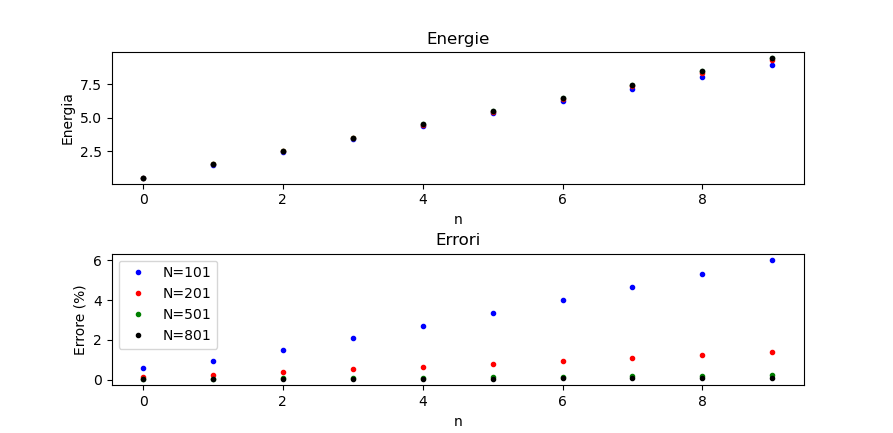
\includegraphics[width=\textwidth]{Differenze.png}
\caption{Variazione dell'errore conseguentemente al numero di punti}
\end{figure}

Dal grafico ottenuto si può vedere che l'errore aumenta ad ogni ulteriore autovalore ricercato, per cui bastano un centinaio di punti per ottenere l'energia più bassa con una deviazione accettabile - inferiore all'un percento - tuttavia le energie superiori, corrispondenti ad $n \ge 1$, presentano divergenze dal risultato analitico che aumentano velocemente verso valori ben superiori. \\
Consideriamo di voler ricavare i primi dieci autovalori: per ottenerli con un errore inferiore all'un percento è necessario arrivare a circa $N=251$, mentre per uno inferiore all'un per mille bisogna giungere a $N=801$. \\
Per quanto riguarda le autofunzioni è invece possibile notare che non vi è variazione significativa nella forma ottenuta, ma che aumentando i punti si ottieme solamente un grafico più rappresentativo.

\begin{figure}[h!]
\centerline{
\begin{minipage}{18cm}
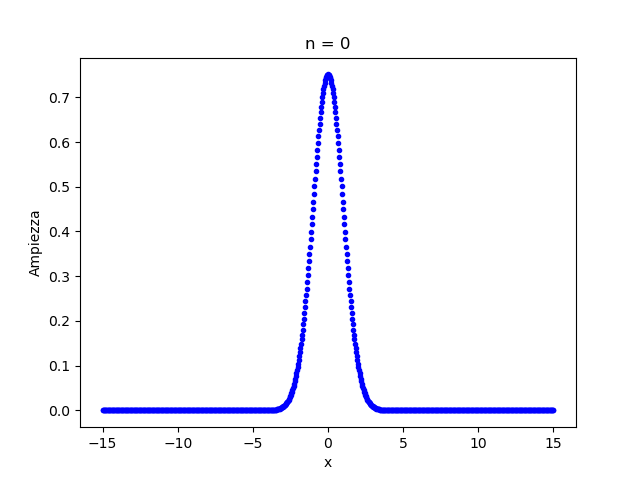
\includegraphics[width=6cm]{auto_A 0.png}  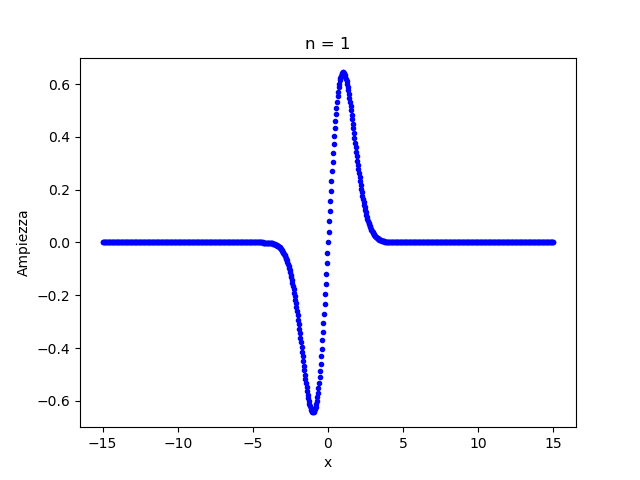
\includegraphics[width=6cm]{auto_A 1.png} 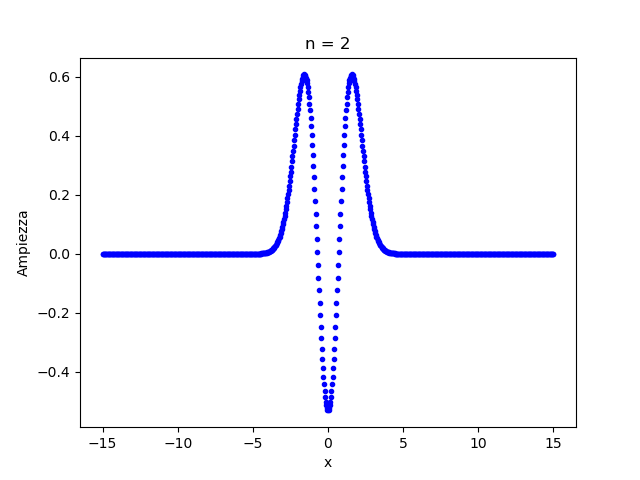
\includegraphics[width=6cm]{auto_A 2.png} \\
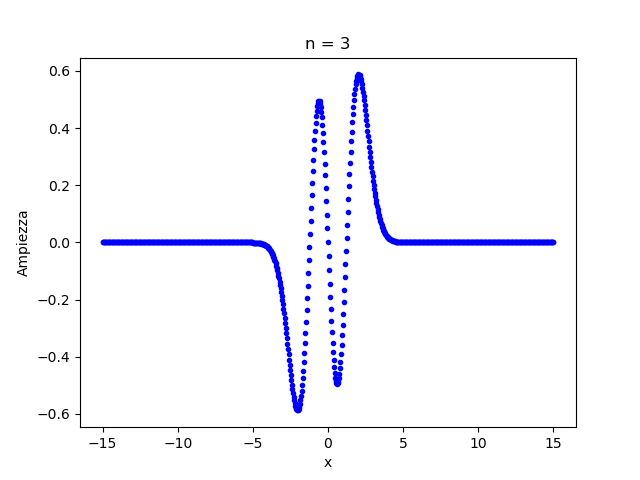
\includegraphics[width=6cm]{auto_A 3.png}  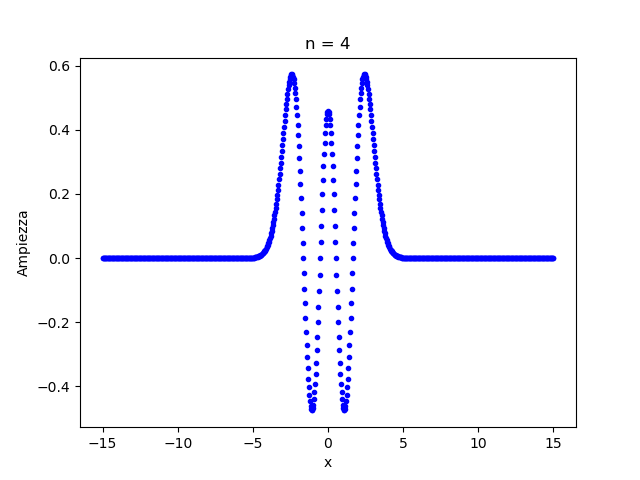
\includegraphics[width=6cm]{auto_A 4.png} 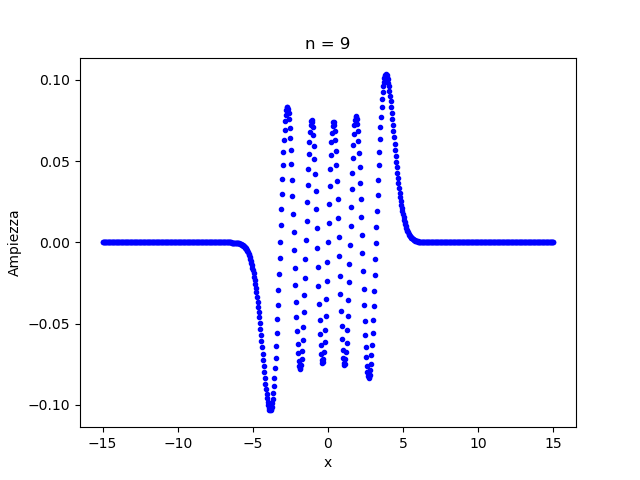
\includegraphics[width=6cm]{auto_A 9.png}
\end{minipage}
}
\caption{Alcune delle autofunzioni per N = 801}
\end{figure}


\subsection*{Task B}

Anche nell'analisi di questo metodo andiamo ad osservare la mutazione dei risultati alla variazione dei parametri. Si può innanzitutto notare l'errore dei risultati è condizionato dall'ampiezza spaziale: essa determina il valore del vettore d'onda e più $L$ è grande, più componenti di Fourier saranno necessari per ottenere autovalori vicini a quelli calcolati analiticamente. \\
Per effettuare un confronto diretto col metodo precedente, poniamo anche in questo caso $L=30$ e analizziamo l'andamento degli errori al variare di $k$, che definisce $2k+1$ componenti di Fourier. \\
Affiché il primo autovalore, corrispondente a $n=0$, abbia associato un errore inferiore all'un percento è necessario che $k$ valga almeno $23$, per un totale di $47$ componenti di Fourier. Con tale valore tuttavia gia il secondo autovalore ha un'errore del tre percento e gli autovalori successivi hanno un'incertezza rapidamente crescente. \\
Consideriamo anche in questo caso i primi dieci autovalori: affiché abbiano tutti un errore inferiore all'un percento sono necessarie 91 componenti. Bastano solo altre dieci componenti affinché, per i medesimi autovalori, l'errore scenda al di sotto dell'un per mille.\\


\begin{figure}[h!]
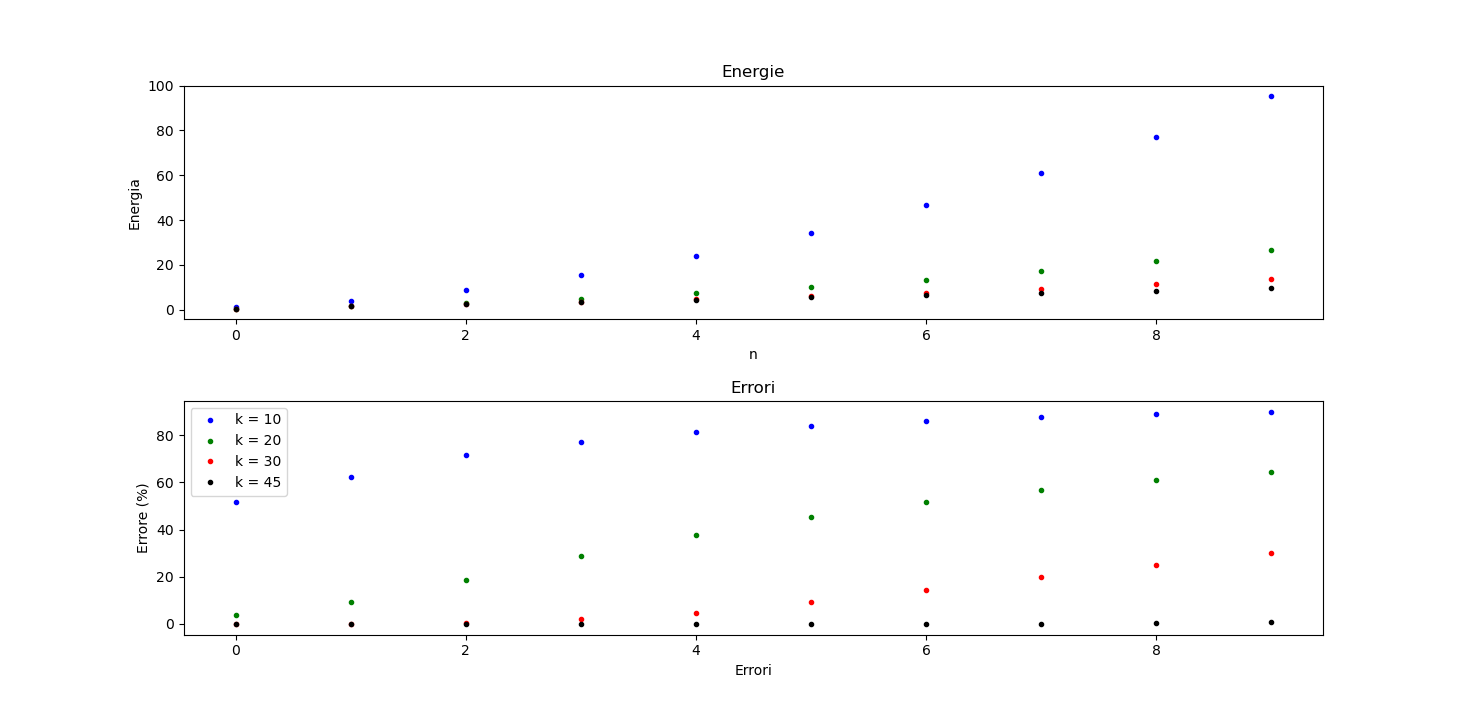
\includegraphics[width=\textwidth]{Differenze_B.png}
\caption{Variazione dell'errore conseguentemente al numero di componenti di Fourier}
\end{figure}


Anche le autofunzioni trovate diventano più precise man mano che $k$ aumenta, infatti un $k$ più alto corrisponde a un numero maggiore di componenti di Fourier che costituiscono la serie. Considerando la terza autofunzione, la differenza della funzione d'onda  fra due casi, $k = 10$ e $k = 40$, è ben evidente: a parità di intervallo spaziale, un numero maggiore di componenti di Fourier determina autofunzioni meno deformate.

\begin{figure}
\centering
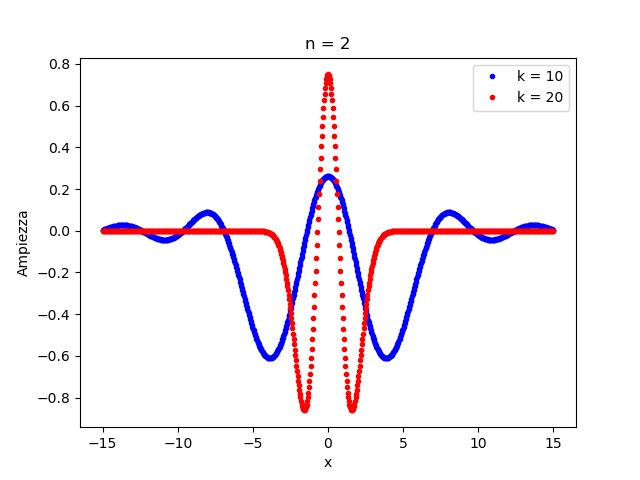
\includegraphics[width=10cm]{fourier.png}
\caption{Confronto di un'autofunzione per due diversi numeri di componenti di Fourier}
\end{figure}

 Il numero di componenti necessarie affinché una data autofunzione non presenti deformazioni significative rispetto alla soluzione esatta risulta essere maggiore al crescere di $n$. Nel caso considerato di errore inferiore all'un per mille, le autofunzioni non presentano già più deformazioni visibili. 
\begin{figure}[h!]
\centerline{
\begin{minipage}{18cm}
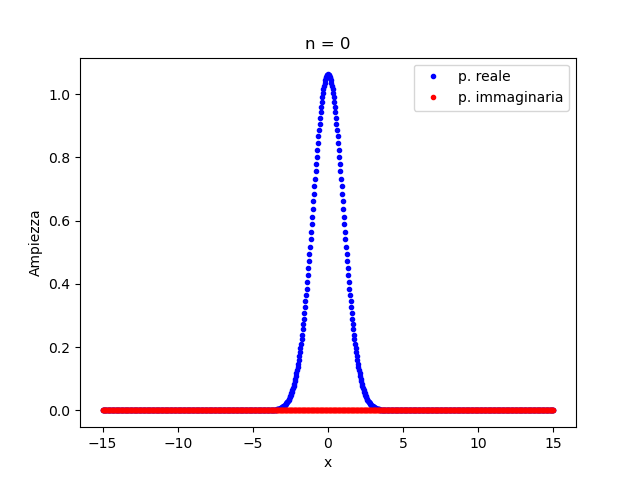
\includegraphics[width=6cm]{auto_B 0.png}  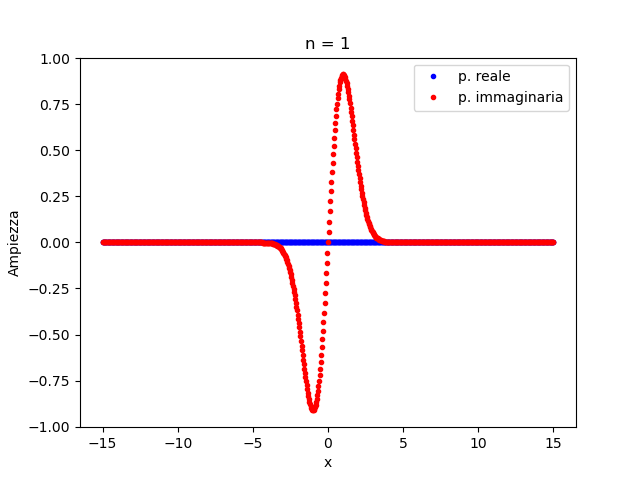
\includegraphics[width=6cm]{auto_B 1.png} 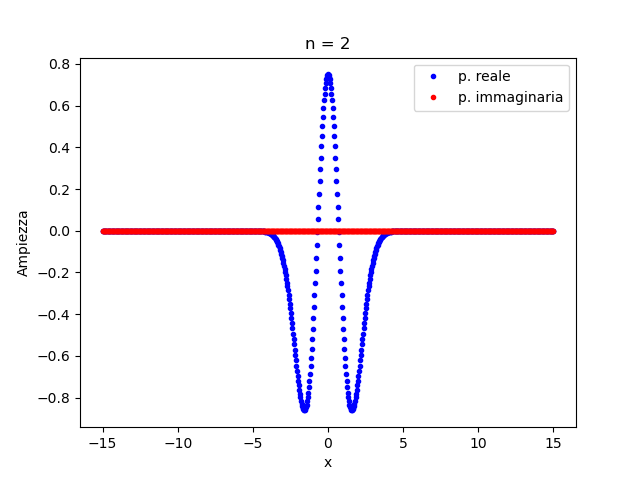
\includegraphics[width=6cm]{auto_B 2.png} \\
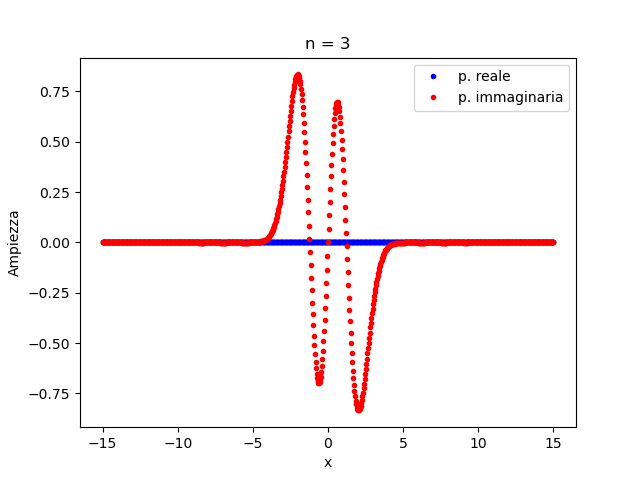
\includegraphics[width=6cm]{auto_B 3.png}  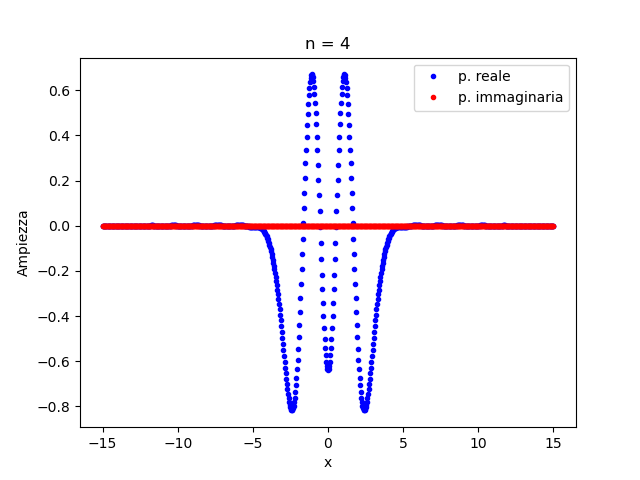
\includegraphics[width=6cm]{auto_B 4.png} 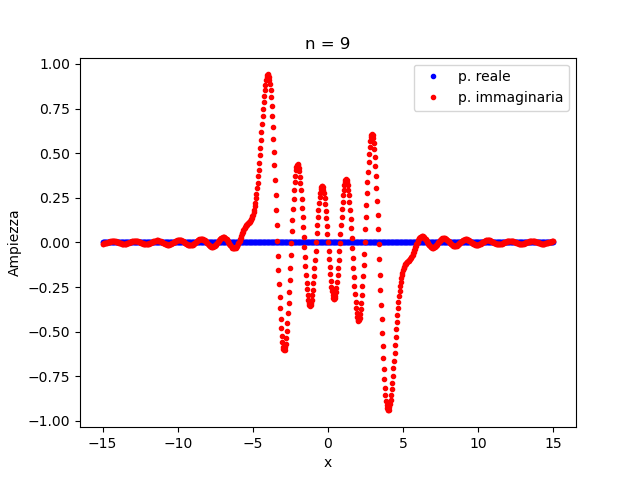
\includegraphics[width=6cm]{auto_B 9.png}
\end{minipage}
}
\caption{Alcune delle autofunzioni trovate con 91 componenti di Fourier}
\end{figure}

\section*{Conclusione}

La potenza dei metodi di diagonalizzazione è dimostrabile anche dall'applicazione a un problema di facile soluzione come quello dell'oscillatore armonico: in entrambi gli approcci seguiti è possibile ottenere risultati estremamente presisi, a patto di considerare un numero sufficientemente elevato di punti o di componenti di Fourier. \\
Il costo computazionale della diagonalizzazione non è elevato. Nel primo metodo, pur avendo una matrice con centinaia di migiaia di elementi, è sufficiente considerare due vettori: uno di dimensione $N$ rappresentane la diagonale principale e uno di dimensione $N-1$ per la sotto-diagonale; nel secondo è necessario lavorare su tutti gli elementi di una matrice $k \times k$, che tuttavia ha una dimensione molto minore della matrice del primo metodo.\\
I tempi di esecuzione mostrano che i due metodi risultano equivalenti, dal momento che \-- considerando il caso di un errore inferiore all'un per mille \-- entrambe le routine impiegano un tempo vicino ai $3 \cdot 10^{-3} s$ oer diagonalizzare le matrici.\\
Entrambi i task forniscono autovalori compatibili con quelli calcolati, ovvero vicini a quantità intere o semi-intere. Vi è accordo anche nella rappresentazione grafica degli autostati, che assumono forma oscillante all'interno della zona permessa e decadono esponenzialmente in quella proibita, così come previsto dalla teoria.

\end{document}
